% Options for packages loaded elsewhere
\PassOptionsToPackage{unicode}{hyperref}
\PassOptionsToPackage{hyphens}{url}
%
\documentclass[
]{article}
\usepackage{amsmath,amssymb}
\usepackage{iftex}
\ifPDFTeX
  \usepackage[T1]{fontenc}
  \usepackage[utf8]{inputenc}
  \usepackage{textcomp} % provide euro and other symbols
\else % if luatex or xetex
  \usepackage{unicode-math} % this also loads fontspec
  \defaultfontfeatures{Scale=MatchLowercase}
  \defaultfontfeatures[\rmfamily]{Ligatures=TeX,Scale=1}
\fi
\usepackage{lmodern}
\ifPDFTeX\else
  % xetex/luatex font selection
\fi
% Use upquote if available, for straight quotes in verbatim environments
\IfFileExists{upquote.sty}{\usepackage{upquote}}{}
\IfFileExists{microtype.sty}{% use microtype if available
  \usepackage[]{microtype}
  \UseMicrotypeSet[protrusion]{basicmath} % disable protrusion for tt fonts
}{}
\makeatletter
\@ifundefined{KOMAClassName}{% if non-KOMA class
  \IfFileExists{parskip.sty}{%
    \usepackage{parskip}
  }{% else
    \setlength{\parindent}{0pt}
    \setlength{\parskip}{6pt plus 2pt minus 1pt}}
}{% if KOMA class
  \KOMAoptions{parskip=half}}
\makeatother
\usepackage{xcolor}
\usepackage[margin=1in]{geometry}
\usepackage{graphicx}
\makeatletter
\def\maxwidth{\ifdim\Gin@nat@width>\linewidth\linewidth\else\Gin@nat@width\fi}
\def\maxheight{\ifdim\Gin@nat@height>\textheight\textheight\else\Gin@nat@height\fi}
\makeatother
% Scale images if necessary, so that they will not overflow the page
% margins by default, and it is still possible to overwrite the defaults
% using explicit options in \includegraphics[width, height, ...]{}
\setkeys{Gin}{width=\maxwidth,height=\maxheight,keepaspectratio}
% Set default figure placement to htbp
\makeatletter
\def\fps@figure{htbp}
\makeatother
\setlength{\emergencystretch}{3em} % prevent overfull lines
\providecommand{\tightlist}{%
  \setlength{\itemsep}{0pt}\setlength{\parskip}{0pt}}
\setcounter{secnumdepth}{5}
\usepackage[german]{babel}
\usepackage{mathtools}
\usepackage{tikz}
\usepackage{pgf}
\usepackage{csquotes}
\AtBeginDocument{
\renewcommand{\maketitle}{}
}
\PassOptionsToPackage{a4paper,margin = 2.5cm}{geometry}
\usepackage{geometry}
\usepackage{float}
\newcommand{\bcenter}{\begin{center}}
\newcommand{\ecenter}{\end{center}}
\renewcommand{\contentsname}{Inhalt}
\usepackage{blindtext}
\usepackage[backend=biber, style = apa]{biblatex}
\addbibresource{Literatur.bib}
\ifLuaTeX
  \usepackage{selnolig}  % disable illegal ligatures
\fi
\usepackage[]{biblatex}
\addbibresource{Literatur.bib}
\usepackage{bookmark}
\IfFileExists{xurl.sty}{\usepackage{xurl}}{} % add URL line breaks if available
\urlstyle{same}
\hypersetup{
  pdftitle={Funktionsweise},
  pdfauthor={Franz Andersch \& Niklas Münz},
  hidelinks,
  pdfcreator={LaTeX via pandoc}}

\title{Funktionsweise}
\author{Franz Andersch \& Niklas Münz}
\date{2024-08-20}

\begin{document}
\maketitle

\subsection{Hard Margin Classifier}

Um das grundlegende Prinzip der SVMs darzustellen gehen wir zuerst von
einer Datensituation aus, in der sich zwei gruppen optimal durch eine
lineare entscheidungsgrenze trennen lassen. Das endgültige Ziel ist es
eine sogenannte Hyperplane zu finden die diese Daten möglichst gut
seperiert und als Entscheidungsgrenze funktioniert. Die allgemeine Form
einer solchen hyperplain lautet \begin{align}
\beta_0+ \beta_1 X_1+\beta_2 X_2+...+\beta_n X_n=0\label{eq:hyperebene}
\end{align} oder in Vektorschreibweise \begin{align}
\overline{\beta}\cdot\overline{x}+\beta_0=0 \label{eq:hyperplanevec}
\end{align} Die geometrische Interpretation des Vektors \(\beta\) und
des Skalars \(\beta_0\) wird in Abbildung \ref{fig:Ebene} im zwei
dimensionalen Fall dargestellt.

\begin{figure}[h]
    \centering
    \begin{minipage}{0.45\textwidth} 
        \centering
        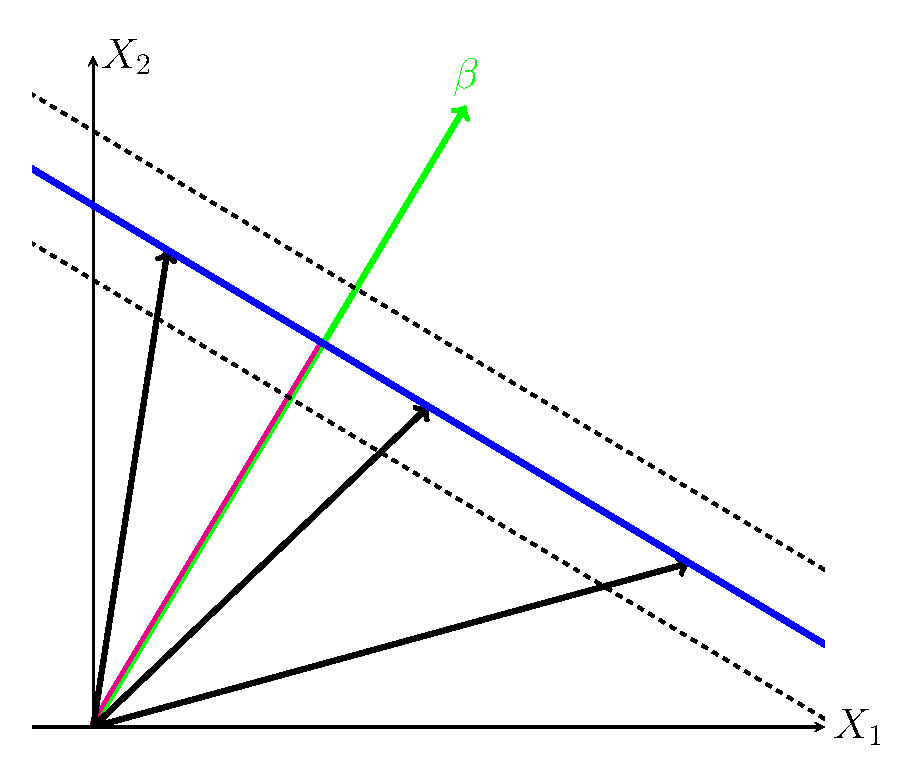
\includegraphics[width=\textwidth,trim=0.5cm 0.5cm 0.5cm 0.5cm]{Images/decision_boundary.pdf} 
        \caption{Konstruktion der Hyperebene}
        \label{fig:Ebene}
    \end{minipage}\hfill
    \begin{minipage}{0.45\textwidth} 
        \centering
        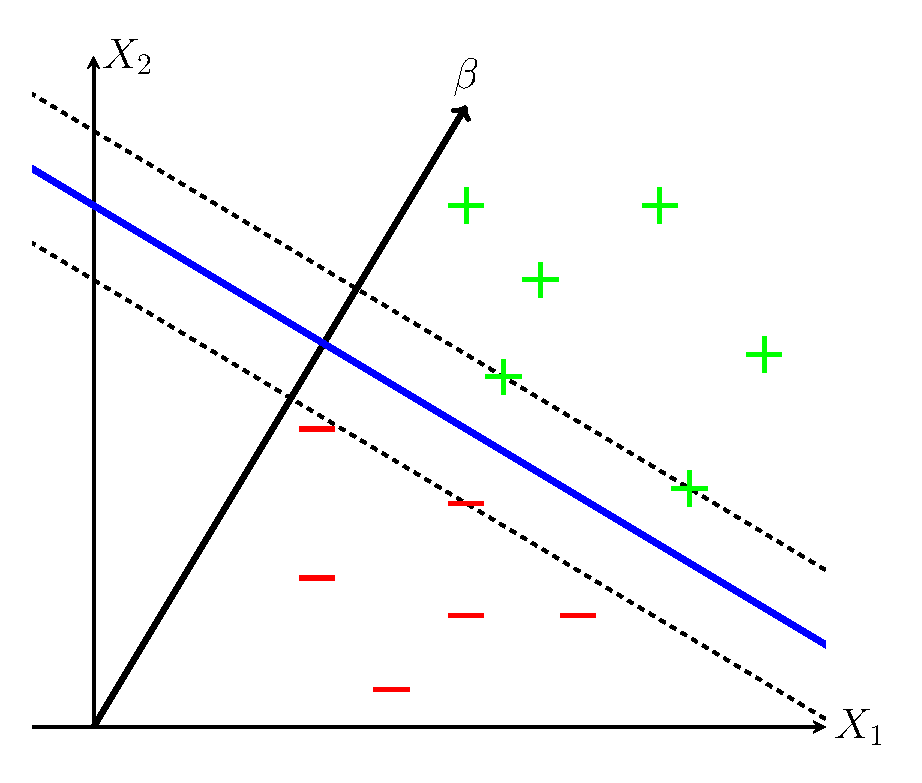
\includegraphics[width=\textwidth,trim=0.5cm 0.5cm 0.5cm 0.5cm]{Images/guttes.pdf}
        \caption{Konstruktion der Margins}
        \label{fig:Margin}
    \end{minipage}
\end{figure}

Die blaue Linie soll die Hyperplain darstellen. Im zweidiemnsionalen
handelt es sich hier um eine Linie. Der \(2 \times 1\) Vektor
\(\overline{\beta}\) liegt immer senkrecht zur konstruierten Hyperplane.
Würde man alle Vektoren, die auf der Hyperplane landen, auf den
\(\overline{\beta}\)-Vektor Projezieren, dann hätten alle diese
Projektionen die selbe Länge \(c\). Also gilt für alle Punkte, die auf
der Ebene liegen. \begin{align}
\frac{\overline \beta}{||\overline{\beta}||}\cdot \overline{x}=c \Leftrightarrow \overline{\beta}\cdot \overline{x}=c \cdot ||\overline{\beta}||\label{eq:betanull}
\end{align} ersetzet man in \eqref{eq:betanull}
\(c \cdot ||\overline{\beta}||\) mit \(-\beta_0\) und zieht dies dann
auf die andere Seite, kommen man wieder bei der ursprünglichen Form aus
Formel \eqref{eq:hyperplanevec} raus.

Als nächstes stellt sich jetzt die Frage, welches \(\overline{\beta}\)
und \(\beta_0\) die optimale Hyperplane darstellen. Betrachtet man die
Abbildung \ref{fig:Margin}, dann ist zu erkennen, dass die Datenpunkte
durch die blaue Linie getrennt werden. Allerdings könnte man
theorethisch undendlich viele andere Hyperplains durch rotation oder
verschiebung konstruieren, die trotzdem die Daten in ihren Ausprägungen
trennen. Um eine eindeutige Lösung zu finden, wird als nächstes ein
bereich um die Hperplane abgesteck. In Abbildung \ref{fig:Margin}
dargestell durch die gestrichelten scharzen linien, welche man als
Schranken bezeichnen könnte. In diesem Bereich sollen keine Datenpunkte
liegen und die Schranken sollen immer parallel zur Hyperplain seien und
den gleichen Abstand zu ihr haben. Außerdem dürfen keine positiven
Samples unterhalb der oberen Schranke liegen und keine negativen
unterhalb. Das gegenteil gilt dementsprechend für die untere Schranke.
Als Definition für die beiden Schranken wird festgelegt \begin{align}
\overline{\beta}\cdot \overline{x}+\beta_0=1\label{eq:posSV}
\end{align} für die Schranke in richtung der grünen Datenpunkte und
\begin{align}
\overline{\beta}\cdot \overline{x}+\beta_0=-1\label{eq:negSV}
\end{align} für die Schranke in Richting der roten Datenpunkte. Aus
dieser Beschränkung für die Hyperplane können wir auch ableiten, dass
für die positiven Samples \(\overline{x}^+\) immer gilt
\(\overline{\beta}\cdot \overline{x}^++\beta_0\ge 1\) und für negative
Samples \(\overline{x}^-\) immer gilt
\(\overline{\beta}\cdot \overline{x}^-+\beta_0\le -1\). Durch einführen
einer weiteren Variable \(y\), welche die eigenschaft hat, dass die den
Wert 1 bei einem positiven und den Wert -1 bei einem negativen Sample
annimmt, können diese zwei Beschränkungen zu einer zusammengefasst
werden \begin{align}
y(\overline{\beta}\cdot \overline{x}+\beta_0)\ge 1\label{eq:Nebenbedingung}
\end{align} Da das Verfahren auch maximum Margin Classifier gennant
wird, gilt es jetzt noch eine Definition für den Margin also den Abstand
zwischen den zwei Schranken zu finden, der schließlich maximiert werden
soll. Damit diese Schranken, maximal weit auseinander liegen, muss es
zwangsläufig Datenpunkte geben, die genau auf den Schranken liegen.
Diese Datenpunkte haben eine wichtige Rolle für die Konstruktion des
Margins. Es sind ausschließlich diese Datenpunkte, die einen Einfluss
auf die finalen werte von \(\overline{\beta}\) und \(\beta_0\) haben
werden. Sie werden \textbf{Support-Vektoren} genannt und geben den SVMs
ihren Namen.

\begin{figure}[h]
\centering
 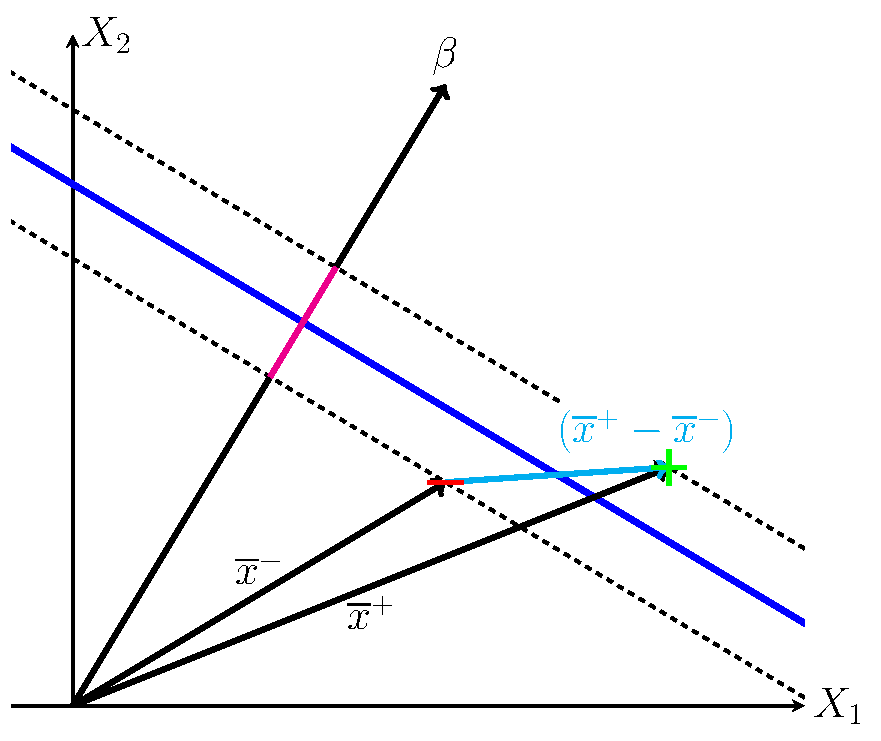
\includegraphics[width=0.5\textwidth,trim=0.5cm 0.5cm 0.5cm 0.5cm]{Images/margin.pdf} 
        \caption{Abhängigkeit des Margins von den Support-Vektoren}
        \label{fig:SupVecs}
\end{figure}

In Abbildung \ref{fig:SupVecs} sind zwei solcher Support-Vektoren zu
einem negativen und positiven Sample dargestellt. Der Margin kann dann
dargestellt werden als eine Projektion dieser Differenz
(\(\overline{x}^+-\overline{x}^+\)) auf den \(\overline{\beta}\)-Vektor.
Damit am Ende die Länge dieses Margins \(M\) rauskommt muss
\(\overline{\beta}\) noch durch seine Länge geteilt werden.
\begin{align}
M=\frac{\overline{\beta}}{||\overline{\beta}||}\cdot \left(\overline{x}^+-\overline{x}^+\right)=\frac{\overline{\beta}\cdot\overline{x}^- -\overline{\beta}\cdot\overline{x}^+}{||\overline{\beta}||}\label{eq:maring1}
\end{align} Es ist bekannt, dass für postive Supportvektoren gilt
\(\overline\beta \overline{x}^+ +\beta_0 = 1 \Leftrightarrow \overline\beta \overline{x}^+=1-\beta_0\)
und für negative
\(\overline\beta \overline{x}^- +\beta_0 = -1 \Leftrightarrow \overline\beta \overline{x}^-=-1-\beta_0\).
Setzt man dies ein in \eqref{eq:maring1}, erhält man als
Maximisierungsziel \begin{align}
M=\frac{1-\beta_0-(-1-\beta_0)}{||\overline\beta||}=\frac{2}{||\overline\beta||}\label{eq:margin2}
\end{align} Um diesen Maximierungsschritt angenehmer zu gestalten, wird
an der Stelle versucht den Ausdruck
\(\frac{1}{2}||\overline \beta||^2=\frac{1}{2}\overline \beta '\cdot \overline \beta\)
zu minimieren. Was im Endeffekt ebenfalls dazu führt, dass der Ausdruck
in \eqref{eq:margin2} maximiert wird.

Dieses Optimierungsproblem mit der Nebenbedingung aus Formel
\eqref{eq:Nebenbedingung} lässt sich am besten über Lagrange-Multiplier
lösen \begin{align}
\mathcal{L}(\overline\beta,\beta_0,\overline \alpha)=\frac{1}{2}\overline \beta ' \overline \beta-\sum \alpha_i[y_i(\overline \beta \cdot \overline{x_i}+\beta_0)-1]\label{eq:Lagrange}
\end{align} Wird dieser Ausdruck partiell abgeleitet und gleich null
gesetzt erhält man als zwischen ergebnis \begin{align}
\frac{\partial \mathcal{L}}{\partial \beta}=\beta-\sum \alpha_i y_i \overline{x_i}\overset{!}{=}0 \Rightarrow \beta=\sum \alpha_i y_i \overline{x_i}\label{eq:solutbeta}
\end{align} somit zeigt sich, dass \(\overline{\beta}\) als
linearkombination der Inputvektoren dargestellt werden kann. Weiterhin
gilt für \(\beta_0\) \begin{align}
\frac{\partial \mathcal{L}}{\partial \beta_0}=\sum \alpha_i y_i \overline{x_i}\overset{!}{=}0\label{eq:solutbeta0}
\end{align} Setzt man dies in \eqref{eq:Lagrange} ein erhält man einen
neuen Ausdruck, denn es gilt zu minimieren \begin{align}
\mathcal{L}(\overline \alpha)=-\frac{1}{2}\sum \sum \alpha_i \alpha_j y_i y_j \overline{x}_i \cdot \overline{x}_j+\sum \alpha_i\label{eq:dualproblem}
\end{align} Die Lösung für diesen Ausdruck erfolgt dann über sogenannte
\enquote{standard non linear optimization algorithms for quadratic forms}
\parencite{boserTrainingAlgorithmOptimal1992}. Nachem für
\(\overline \alpha\) gelöst wurde, kann dies in \eqref{eq:solutbeta}
eingesetzt werden um das optimale \(\overline{\beta}\) zu erhalten. Es
kann gezeigt werden, dass die gelösten \(\alpha_i\) lediglich für die
Supportvektoren werte ungelich Null annehmen. Somit ist der
Koeffizientenvektor \(\overline{\beta}\) sogar eine Linearkombination
von nur den Supportvektoren
\parencite{boserTrainingAlgorithmOptimal1992}. Die letzte unbekannte
\(\beta_0\) kann gelöst werden, indem man mithilfe von einem
positiven/negativen Support Vektor \eqref{eq:posSV}/ \eqref{eq:negSV}
nach \(\beta_0\) löst.

Mit den gelösten Werten zur optimalen Hyperplane kann jetzt auch eine
Entscheidungsregel für ungelabelte Datenvektoren \(\overline{x}_u\)
konstruiert werden. Bedenkt man also wenn man einen Vektor der nicht auf
der Hypeplane liegt in \eqref{eq:betanull} einsetzt erhält man also
\(\frac{\overline \beta}{||\overline{\beta}||}\cdot \overline{x}_u=c+k\).
Wenn \(k\) positiv ist, liegt der neue Datenpunkt oberhalb der
Hyperplane liegt und somit als positives Sample gewertet wird. Wenn
\(k\) negativ ist, dann liegt der Datenpunkt unterhalb der Hyperplane
und wird als negativ gewertet. Mit der gleichen Umformung wie weiter
oben schon beschrieben kommt man zu folgender Entscheidungsregel
\begin{align}
f(\overline{x}_u)=\begin{cases}\mathrm{positiv}&\text{wenn } \overline{\beta}\cdot \overline{x}_u+\beta_0 > 0\\
\mathrm{negativ} & \text{wenn }\overline{\beta}\cdot \overline{x}_u+\beta_0<0
\end{cases}\label{eq:decisionf}
\end{align}

\subsection{Soft Margin Classifier}

Dass die Daten sich perfekt linear trennen lassen ist zwar ein gut um
die Vorgehensweise zu veranschaulichen, tritt aber in realen Situationen
so gut wie nie auf. Falls sich postitive und negative Samples im Raum
überlappen, ist die Konstruktion einer Hyperplane wie beim Hard Margin
Classifier unmöglich. Man müsste also entweder auf eine nicht lineare
Hypeplane ausweichen oder man erweicht die vorgaben für die Konstruktion
der Hyperplane. Zweiteres ist genau das, was durch die Soft Margin
Classifier erreicht wird. Die Vorgabe für die Konstruktion der Schranken
ermöglicht es einzelnen Datenpunkten auf der falschen Seite der
Schranke, ja sogar der Entscheidungsgrenzen zu liegen. Dafür wird für
die Einschränkungen eine sogennannte Slackvariable \(\varepsilon\)
eingeführt \parencite{jamesIntroductionStatisticalLearning2021}. Setzt
man diese in diese in \eqref{eq:Nebenbedingung} lautet die neuen
Nebenbedingung \begin{align}
y_i(\beta \cdot \overline{x}_i-\beta_0)>1- \varepsilon_i \label{eq:nebbedsfm}
\end{align}

\begin{figure}[h]
\centering
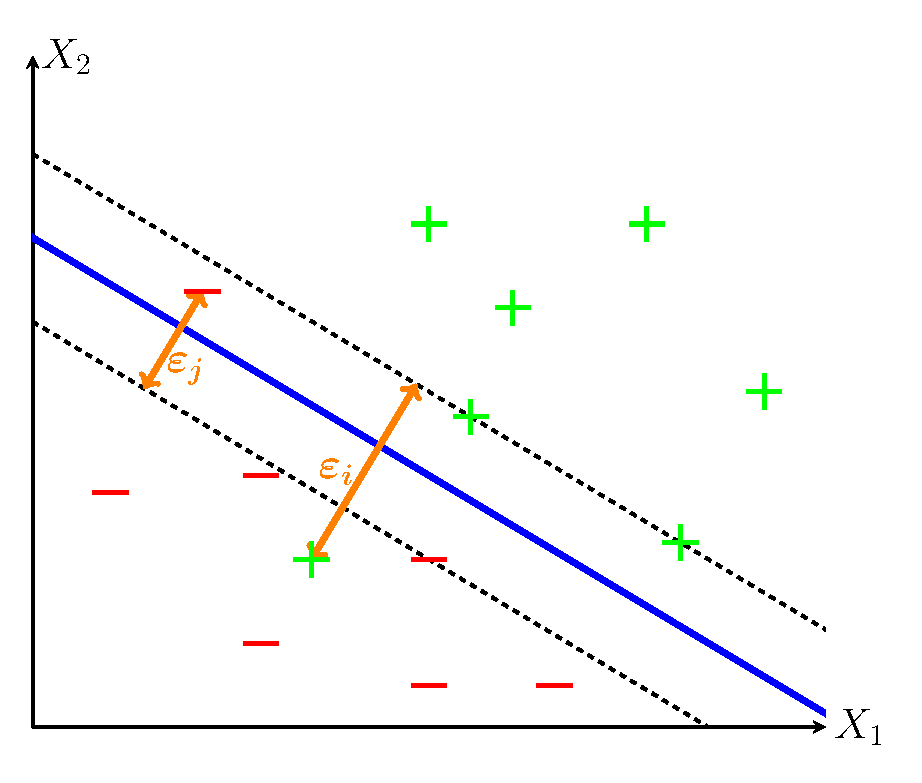
\includegraphics[width=0.5\textwidth,trim=0.5cm 0.5cm 0.5cm 0.5cm]{Images/slackvariable.pdf} 
        \caption{Funktion der Slack Variable}
        \label{fig:slackvariable}
\end{figure}

Jetzt könnte man versuchen diese neue Nebenbedingung einfach in das
zuvor angewandte Optimisierungsverfahren einzufügen. Allerdings besteht
hier das Problem, dass \(\varepsilon\) einfach immer maximal groß
gewählt wird und so die Bedingung immer erfüllt wird. Um das Ausmaß der
Verletzung der usptünglichen Annahmen zu begrenzen, aber trotzdem noch
gewisse Abweichung zuzulassen, wird ein weitere Parameter \(C\)
eingeführt, als regularisierender Parameter für \(\varepsilon\). Leitet
daraus zusammen mit der Restriktion \(\varepsilon\ge0\) wieder einen
Lagrangefunktion her erhält man \begin{align}
\mathcal{L}(\overline\beta,\beta_0,\overline\alpha,\overline\varepsilon,\overline\lambda)=\frac{1}{2}\overline\beta'\cdot \overline\beta + C \sum_{i=1}^{n}\varepsilon_i-\underbrace{\sum \alpha_i[y_i(\overline\beta \cdot \overline{x_i}+\beta_0)-1+\varepsilon_i]}_{\text{für }y_i(\overline\beta \cdot \overline{x}_i-\beta_0)>1- \varepsilon_i}-\underbrace{\sum \lambda_i \varepsilon_i }_{\substack{\text{für}\\ \varepsilon_i \ge 0}}
\end{align} Wenn dieser Ausdruck wie beim Hardmargin Classifier gelöst
wird und die Ergebnisse eingesetzt werden erhält man wieder den Ausruck
aus \eqref{eq:dualproblem} mit der zusätzlichen Einschränkung
\(0\le \alpha_i \le C\). Dieses Maximierungsproblem wird dann genauso
aufgelöst wie bei dem Hard Margin Classifier und die Entscheidungsregel
ist ebenfalls gleich.

\subsection{Der Kernel Trick}

Auch wenn eine lineare Entscheidungsgrenze Vorteile in Sachen
Generalisierbarkeit bietet, ist sie doch nicht für jede Datensituation
geeignet.In Abbildung \ref{fig:nonlinearsep} ist es sehr gut zu
erkennen, dass in diesem Fall eine lineare Grenze zwischen den Klassen
keinen Sinn Ergeben würde und eine elliptische Form wahrscheinlich
besser geeignet wäre. Eine Lösung für dieses Problem, wäre den
Merkmalsraum zu erweitern. So könnte die angenommene Formel für die
lineare Hyperebene in \eqref{eq:hyperebene} durch polynomterme der
Merkmale \(X_i\) oder durch Interaktionstherme erweitert werden. Dies
führt dazu, dass die Entscheidungsgreze in diesem vergrößerten
Merkmalsraum immer noch linear ist, aber die Trennung möglich ist (siehe
Abbildung \ref{fig:featurexten}). Transformiert man diese dann wieder in
den ursprünglichen Merkmalsraum ist die Entscheidungsgrenze dann nicht
mehr linear. Allerdings führt diese Herangehensweise zu eine starken
Anstieg des Rechenaufwands, da die Möglichkeiten der Merkmalserweiterung
endlos sind \parencite{jamesIntroductionStatisticalLearning2021}.

Die Lösung für das Problem sind sogenannte Kernel Funktionen. Betrachtet
man die entscheidungsfunktion \eqref{eq:decisionf} und setzt für
\(\overline{\beta}\) die Gleichung aus \eqref{eq:solutbeta} erhält man
\begin{align}
f(x_u)= \sum \alpha_i y_i x_i \cdot x_u +\beta_0
\end{align} Es zeigt sich also, dass die Entscheidungsfunktion im
Wesentlichen aus einer Linearkombiantion von Punktprodukten aus dem
Vektor \(x_u\) mit allen Trainingsvektoren \(x_i\) ergibt. Diese
Punktprodukt kann als Ähnlichkeitsmaß zwischen dem neuen Datenpunkt und
dem jeweiligen Trainingsdatenpunkt interpretiert werden. Es ist nun
Möglich diese Produkte durch eine Funktion zu ersetzen, welche die
Ähnlichkeiten von Datenpunkten anders bewertet. Diese sogenannte Kernel
Funktion \(K(x_i,x_j)\) ermöglicht es eine flexiblere
Entscheidungsgrenze zu implementieren. Der Vorteil ist dabei, dass die
Kernel Funktion nur auf alle Punktprodukte angewndet wird und es dabei
nicht nötig ist den Merkmalsraum zu Erweitern, was wiederum Rechenzeit
spart\parencite{jamesIntroductionStatisticalLearning2021}. Die
Entscheidungsfunktion wird dann mithilfe dieser Kernelfunktionen
berechnet: \begin{align}
  f(x_u)=\sum \alpha_i y_i K(x_i,x_u)+\beta_0
\end{align}

\begin{figure}[h]
    \centering
    \begin{minipage}{0.45\textwidth} 
        \centering
        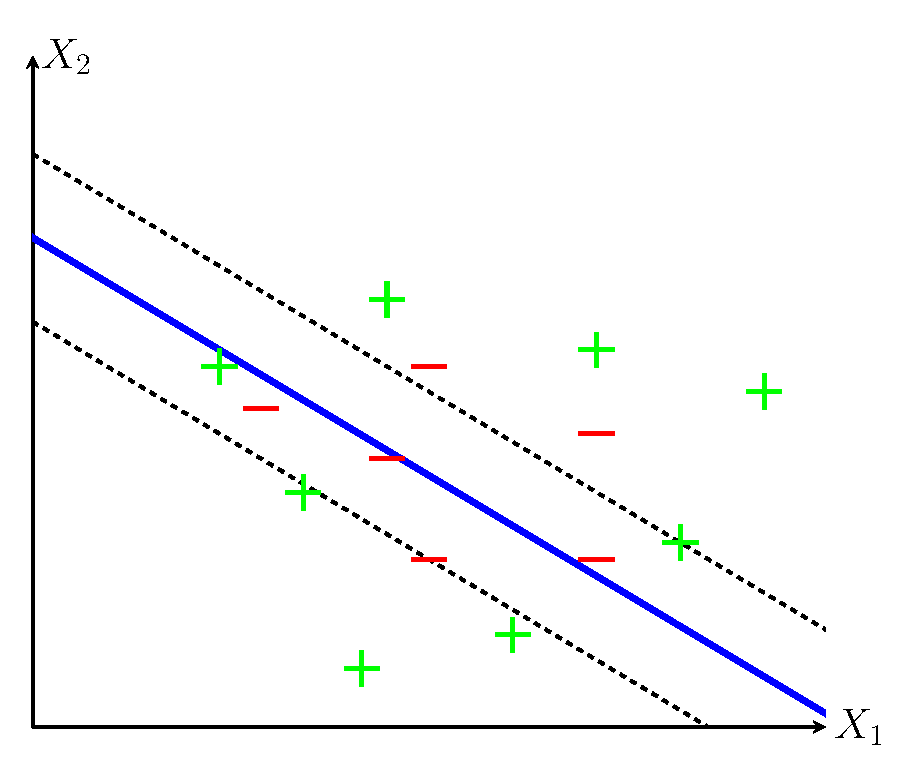
\includegraphics[width=\textwidth,trim=0.5cm 0.5cm 0.5cm 0.5cm]{Images/nonlinearseperable.pdf} 
        \caption{nicht linear getrennte Daten}
        \label{fig:nonlinearsep}
    \end{minipage}\hfill
    \begin{minipage}{0.45\textwidth} 
        \centering
        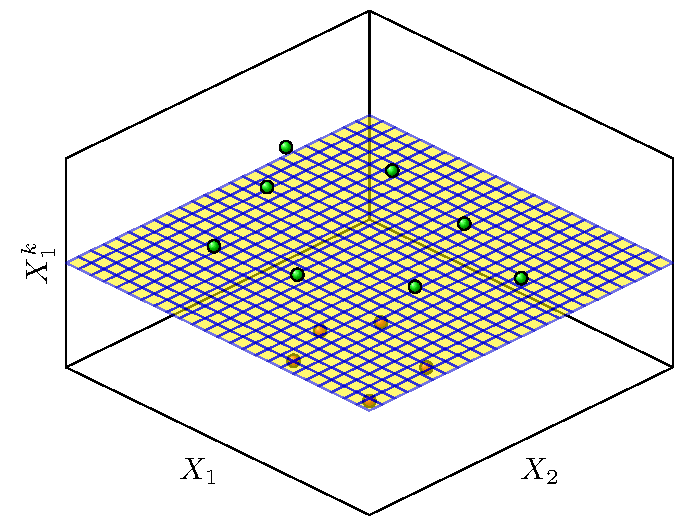
\includegraphics[width=\textwidth,trim=0.5cm 0.5cm 0.5cm 0.5cm]{Images/featurexpansion.pdf}
        \caption{Feature Erweiterung}
        \label{fig:featurexten}
    \end{minipage}
\end{figure}

Es gibt eine ganze Reihe an Kernelfunktionen, die bei SVMs Anwedung
finden. Die Grundlage ist der lineare Kernel, wobei dieser lediglich das
Punktprodukt beschreibt, also praktisch genau das macht, was bei einer
linearen Entscheidungsgrenze gemacht wird. Deweiteren gibt es den
Polynomial Kernel. Dieser hat die Form \begin{align}
 K(x_i,x_u)=(1+x_i\cdot x_u)^d
\end{align} Die Verwendung von diesem Kernel führt dazu, dass die
Entscheidungsgrenze sich ähnlich Verhält, wie als würde man zu Beginn
eine Merkmalserweiterung mit Polynomen vom Grad \(d\) durchführen (siehe
Abbildung \ref{fig:polykernel}. Eine weitere Kernel Funktion ist der
Radial Basis Function Kernel(RBF) mit der Form \begin{align}
K(x_i,x_u)=\exp\left(-\gamma ||x_i-x_u||^2\right)
\end{align} Für diesen Kernel wird die quadrierte euklidische Distanz
als Ähnlichkeitsmaß verwendet, was dazu führt, dass für diejenigen
\(x_i\) die näher an \(x_u\) liegen, in der Entscheidungsfunktion einen
größeren Einfluss haben. Der Parameter \(\gamma\) legt dann fest, wie
stark der Einfluss der Distanz sein soll. Die projektion die der Kernel
hier macht ist eine, in einen uendlich großen Merkmalsraum . Daher
könnte man selbst durch vorgeriges Erweitern des Merkmalsraums nicht das
Ergebnis eines RBF Kernel replizieren und dies führt auch zu einer sehr
flexiblen Entscheidungsgrenze (siehe Abbildung \ref{fig:radialkernel})\\

\begin{figure}[H]
    \centering
    \begin{minipage}{0.45\textwidth} 
        \centering
        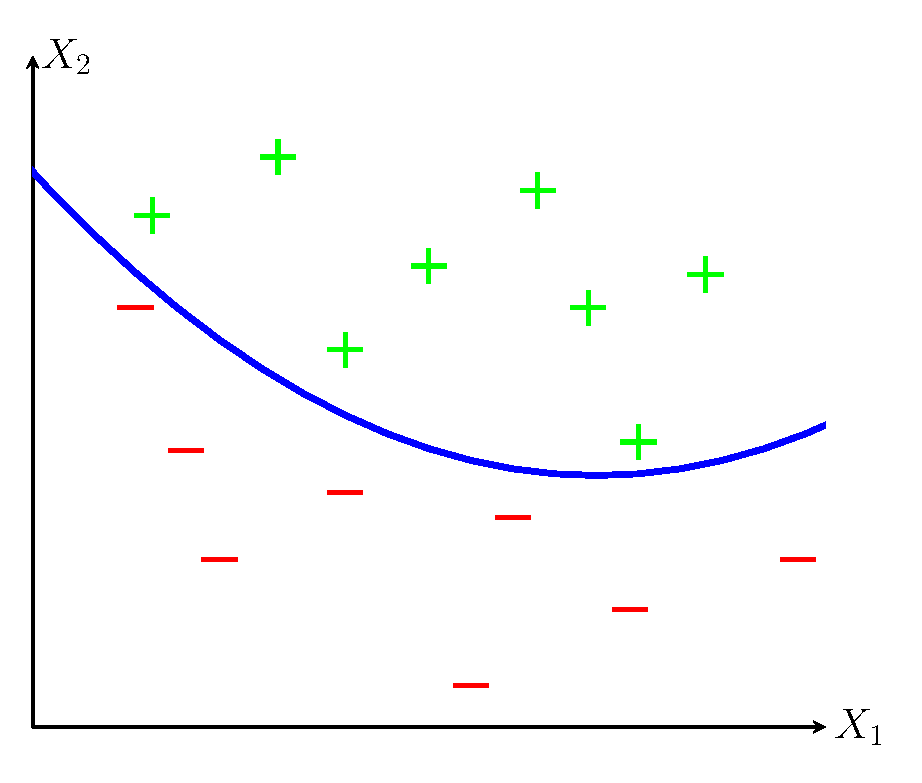
\includegraphics[width=\textwidth,trim=0.5cm 0.5cm 0.5cm 0.5cm]{Images/ploynomial kernel.pdf} 
        \caption{Mögliche Entscheidungsgrenze für polynomial Kernel}
        \label{fig:polykernel}
    \end{minipage}\hfill
    \begin{minipage}{0.45\textwidth} 
        \centering
        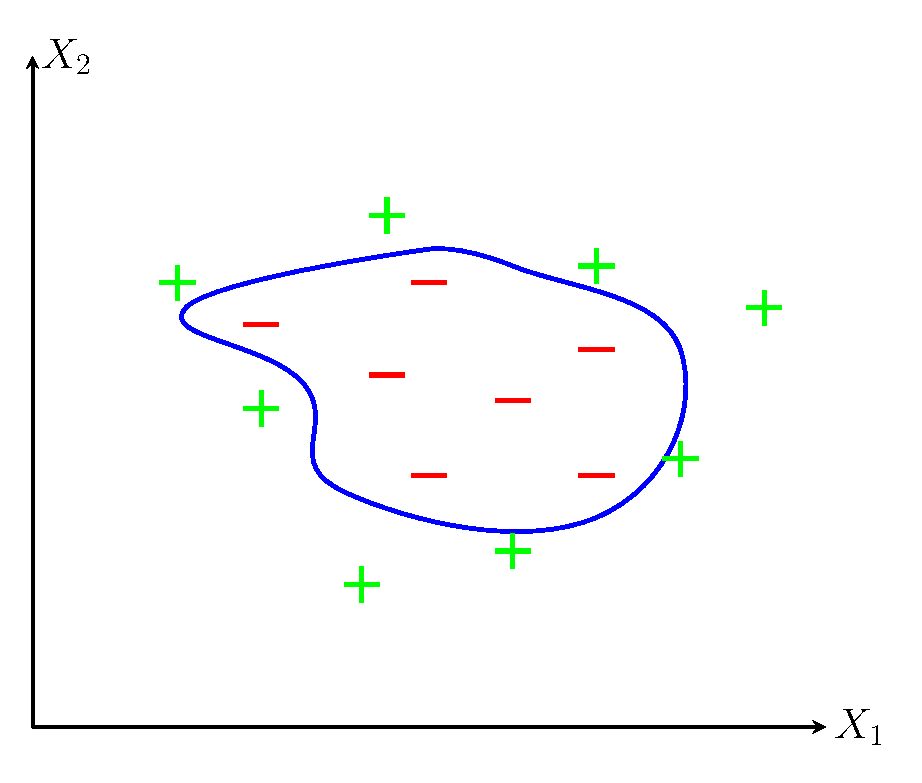
\includegraphics[width=\textwidth,trim=0.5cm 0.5cm 0.5cm 0.5cm]{Images/radial_kernel.pdf}
        \caption{Mögliche Entscheidungsgrenze für RBF Kernel}
        \label{fig:radialkernel}
    \end{minipage}
\end{figure}

Es gibt noch einen Reihe wietere Kernel, die auf unterschiedlichen
Ähnlichkeitsmaßen beruhen, aber eher seltener oder nur in speziellen
Zusammenhänge angewendet werden. Wichtig ist anzumerken, dass die
Verwendung von Kernels zwar die Flexibilität der Entscheidungsgrenze
erhöht, damit aber auch die Gefahr von overfitting einhergeht.
Zusätzlich werden mit den Kernels auch neue Hyperparameter wie \(d\)
oder \(\gamma\) eingeführt, die bei der Model selektion ebenfalls
beachtet werden müssen.

\printbibliography

\end{document}
